\label{sec:evaluation}

All evaluations are performed on a quiescent Intel Core 2 dual-processor system equipped with 
16GB RAM. 
Each processor is a 4-core 64-bit Intel Xeon running at 2.33 GHz with a 4MB
shared L2 cache and 32KB private L1 cache. 
The underlying operating system is unmodified CentOS 5.5, running with Linux kernel
version 2.6.18-194.17.1.el5. The glibc version is 2.5. 
In order to compare performance fairly, all benchmarks were built as 64-bit executables 
using LLVM compiler (clang-3.2). The compiler optimization level is set to ``-O1'' 
so memory allocation callsites can be reported precisely.
%since we can not report line number of source code with optimization level larger than
%``-O2''.
In our evaluation, we use two popular benchmark suites,
Phoenix (with large input) ~\cite{phoenix-hpca} and PARSEC (with simlarge input) ~\cite{parsec}. Even with unmodified LLVM-3.2, Facesim can not be compiled successfully (with complaints on an undefined template) and Canneal aborts unexpectedly. Thus, Facesim and Canneal are excluded here. 

This evaluation aims to answer the following questions:
\begin{itemize}
\item
  How effective is \Predator{} at detecting and predicting false sharing (Section~\ref{sec:effective})?

\item
  What is the performance and memory overhead of \Predator{} with and without prediction
  (Sections~\ref{sec:perfoverhead} and \ref{sec:memoverhead})?

\item 
  \CC{How sensitive is \Predator{} on different thresholds and sampling rate (Section~\ref{sec:sensitivity})}? 
 
\end{itemize}

\subsection{Detection and Prediction Effectiveness}
\label{sec:effective}

As discussed in Section~\ref{sec:runtime}, \Predator{} can precisely report  
false sharing problems. 
Figure~\ref{fig:lrreport} shows an example report generated by \Predator{} for the \texttt{linear\_regression} 
benchmark. From this report, we can see that false sharing is caused by a heap object, which
has a large number of cache invalidations. 
The callsite stack is also listed in this report. \Predator{} also reports word level access information
of this object. This information lets us see that there is no \emph{current} false sharing problem, because different threads are accessing different cache lines. However, \Predator{} has predicted that this program does 
have a latent false sharing problem, which would be exposed if the starting address of this object were different. 

\begin{figure*}[!ht]
{\centering
\subfigure{\lstinputlisting[numbers=none,frame=none,boxpos=t]{fig/linearregression.report}}
\caption{False sharing report for the \texttt{linear\_regression} benchmark.
\label{fig:lrreport}}
}
\end{figure*}



\subsubsection{Benchmarks}
\label{sec:benchmarks}
Results on two benchmark suites, Phoenix and PARSEC, are listed in the Table~\ref{table:detection}. 

%Our results show that \Predator{} not only capture previously-discovered
%false sharing, but also many detect new false sharing places. The results
%are listed in Table~\ref{table:detection}. 

%http://www.technovelty.org/tips/getting-a-tick-in-latex.html
%http://tex.stackexchange.com/questions/42619/x-mark-to-match-checkmark
%\begin{comment}
\begin{table*}[ht!]
{\centering\begin{tabular}{l|r|r|r|r|r}\hline
{\bf \small Benchmark} & {\bf \small Source Code} & {\bf \small New} & {\bf \small Without Prediction} &{\bf \small With Prediction} & {\bf \small Improvement} \\
\hline
\small \textbf{histogram} & {\small histogram-pthread.c:213} & \cmark{} &\cmark{} & \cmark{} & 46.22\%\\
\small \textbf{linear\_regression} & {\small linear\_regression-pthread.c:133} & & & \cmark{} & 1206.93\% \\
\small \textbf{reverse\_index} & {\small reverseindex-pthread.c:511} & & \cmark{} & \cmark{} & 0.09\%\\
\small \textbf{word\_count} & {\small word\_count-pthread.c:136} & & \cmark{} & \cmark{} & 0.14\%\\
\hline
\small \textbf{streamcluster} & {\small streamcluster.cpp:985} &  & \cmark{} & \cmark{} &7.52\% \\
\small \textbf{streamcluster} & {\small streamcluster.cpp:1907} & \cmark{} & \cmark{} & \cmark{} & 4.77\%\\
\hline
\end{tabular}
\caption{Detection results of \Predator{} on Phoenix and PARSEC benchmark suites. \label{table:detection}}
}
\end{table*}

In this table, the first column lists those programs with false
sharing problems.  The second column shows precisely where the problem
is. Since all discovered false sharing occurs inside the same heap
object, we list callsite source code information in this column.  The
third column ``New'' marks whether this false sharing was newly
discovered by \Predator{} or not.  A checkmark in the appropriate
column indicates whether the false sharing was identified without
prediction and/or with prediction.  The final column, ``Improvement'',
shows the performance improvement after fixing false sharing.
%The number is based on the average runtime of $10$ runs. 

As shown in the table, \Predator{} reveals several unknown false sharing problems. 
It is the first tool to detect these two false sharing problems: one in \texttt{histogram} 
and one in line $1908$ of \texttt{streamcluster}. 
In \texttt{histogram}, multiple threads repeatedly modify different locations of the same heap object. 
Padding the data structure \texttt{thread\_arg\_t} fixes the false sharing problem and 
helps to improve the performance around 46\%.
In \texttt{streamcluster}, multiple threads are simultaneously accessing and updating 
the same \texttt{bool} array, \texttt{switch\_membership}. 
By simply changing this array to \texttt{long} type contributes to about 4.7\% performance improvement.

%, although it is not a complete fix of false sharing. 
%None of these two false sharing problems has been reported by previous tools.
All other false sharing problems have been discovered by previous tools~\cite{sheriff}.
We do not see much performance improvement for \texttt{reverse\_index} and 
\texttt{word\_count} benchmarks, but the number of cache invalidations 
among them reaches our predefined threshold so they are reported by \predator{}.
Making reporting threshold higher can avoid the report of insignificant false sharing problems.
It is worth noting that these two benchmarks definitely have false sharing problems,
which has been confirmed by \Sheriff~\cite{sheriff}. 
We also confirm this manually. 

\texttt{streamcluster} has another false sharing problem at line $985$. 
Different threads change the same object (\texttt{work\_mem}) simultaneously. 
Authors of \texttt{streamclsuter} have already realized possible
false sharing problems and meant to utilize a macro \texttt{CACHE\_LINE} to avoid it. Unfortunately,
the defaulted value of this macro is set to $32$ bytes, which is different with the actual
cache line size of our hardware. By setting to $64$ bytes instead, we achieve around $7.5\%$ performance
improvement.

\texttt{linear\_regression} has a severe false sharing problem, 
while fixing it improves the performance more than $12\times$.
In this benchmark, different threads update their thread specific locations 
inside a heap object(\texttt{tid\_args}) in a tight loop, 
causing a huge amount of cache invalidations. 
For this benchmark, Nanavati et al.~\cite{OSdetection} have observed that 
false sharing occurs when using clang
disappears when using gcc with optimization levels -O2 and -O3.  
But their observation is different with our evaluation. 
During our evaluation, because our customized memory manager has different allocation 
metadata for each heap object, this false sharing does not 
occur at all when we are compiling this program
using \texttt{clang-3.2} at ``-O1'' optimization level.
Thus, \Predator{} actually cannot detect this false sharing problem without enabling its
prediction mechanism, which is discussed in detail in Section~\ref{sec:predicteval}.
Using the prediction mechanism discussed in Section~\ref{sec:prediction},
\Predator{} can detect the false sharing problems in this benchmark.

\subsubsection{Real Applications}
To verify its practicality, we further evaluate \Predator{} 
on several widely-used real applications, whereas no previous work has done this.  
These real applications include a server application (MySQL~\cite{mysql}),
a standard C++ library (Boost~\cite{libfalsesharing}),
a distributed memory object caching system (\texttt{memcached}), a network retriever (\texttt{aget}),
a parallel bzip2 file compressor (\texttt{pbzip2}), and a parallel file scanner (\texttt{pfscan}).
For MySQL and Boost,
we evaluate two specific versions, MySQL-5.5.32 and
boost-1.49.0, which are known to have some false sharing problems.
The specific versions of the other applications are memcached-1.4.15,
aget-0.4.1 and {pbzip2-1.1.6}.

The false sharing problem of MySQL has caused a significant scalability problem and
was very difficult to identify.
According to the architect of MySQL Mikael Ronstrom, ``we had gathered specialists on 
InnoDB..., participants from MySQL support... and a number of generic specialists on 
computer performance...'', ``the fruit of the meeting ... were able to 
improve MySQL performance by 6$\times$ with those scalability fixes''~\cite{mysql}. 
The false sharing of boost library is caused by the special usage of \texttt{spinlock} pool.
Different threads may utilize different spinlocks located in the same cache line in this case.
Fixing it brings a 40\% performance improvement.
\Predator{} is able to successfully detect false sharing locations
in both MySQL and the Boost library. 
For the other four applications, \Predator{} does not find severe false sharing problems.

\subsubsection{Prediction Effectiveness}
\label{sec:predicteval}
We have discussed that prediction helps to reveal the false sharing problems inside \texttt{linear\_regression} benchmark. In this section, we further verify whether prediction can always identify 
false sharing problems even without occurrences.
\texttt{linear\_regression} benchmark is selected here because of the following two reasons:
\begin{enumerate}
\item
The false sharing problem of this benchmark cannot be detected without prediction; see Section~\ref{sec:benchmarks}. 

\item
False sharing severely degrades performance when it actually occurs. 
Hence, it is a serious problem that should always be detected. 
\end{enumerate}

\begin{figure}[!ht]
{\centering
\subfigure{\lstinputlisting[numbers=none,frame=none,boxpos=t]{fig/linearregression.psedocode}}
\caption{False sharing problem inside \texttt{linear\_regression} benchmark.
\label{fig:linearregression}}
}
\end{figure}

Figure~\ref{fig:linearregression} shows the data structure and source code
experiencing false sharing.
The size of this data structure, \texttt{lreg\_args}, is $64$ bytes 
when we use clang to compile a $64$-bit binary at the ``-O1'' optimization level.
For this false sharing problem, the main thread allocates an array with the number of elements equalling
that of the number of underlying hardware cores.
Each element is a \texttt{lreg\_args} type with $64$ bytes. 
Then this array is passed to different threads (\texttt{lreg\_thread}) 
so that each thread only updates its thread-dependent area, see Figure~\ref{fig:linearregression}.
False sharing occurs if two threads happens to update data in the same cache line. 
However, different fields of \texttt{lreg\_args} has different access pattern:
only those fields between $SX$ and $SXY$ (totally around $40$ bytes) are constantly read and updated.
Consequently, the performance of \texttt{linear\_regression} is very sensitive to 
the starting address of false sharing object (see Figure~\ref{fig:perfsensitive}),
which can be changed by many dynamic properties according
to the discussion in Section~\ref{sec:intro}.

Figure~\ref{fig:perfsensitive} shows performance sensitivity to 
offsets of the starting address between the false sharing object and corresponding cache lines. 
When the offset is $0$ or $56$ bytes, this benchmark achieves its optimal performance 
and has no false sharing at all.
When the offset is $24$ bytes, this benchmarks runs around $15$ times slower 
than its optimal performance because of false sharing problem.
When we evaluate detection effectiveness on its original code in Section~\ref{sec:benchmarks}, 
our customized memory manager happens to make the offset $56$ bytes. 
As a result, \Predator{} can not detect false sharing in this benchmark 
without enabling prediction because false sharing does not occur.
This situation happens to all existing tools: they can only detect false sharing problems when
they occur. 

In contrast, the prediction mechanism designed in \predator{} 
aims to address this problem. Our evaluations show 
that \Predator{} can always predict the false sharing problem in this
benchmark no matter what the offset value is, demonstrating its effectiveness.

\subsection{Performance Overhead}
\label{sec:perfoverhead}

\begin{figure*}[ht]
\begin{center}
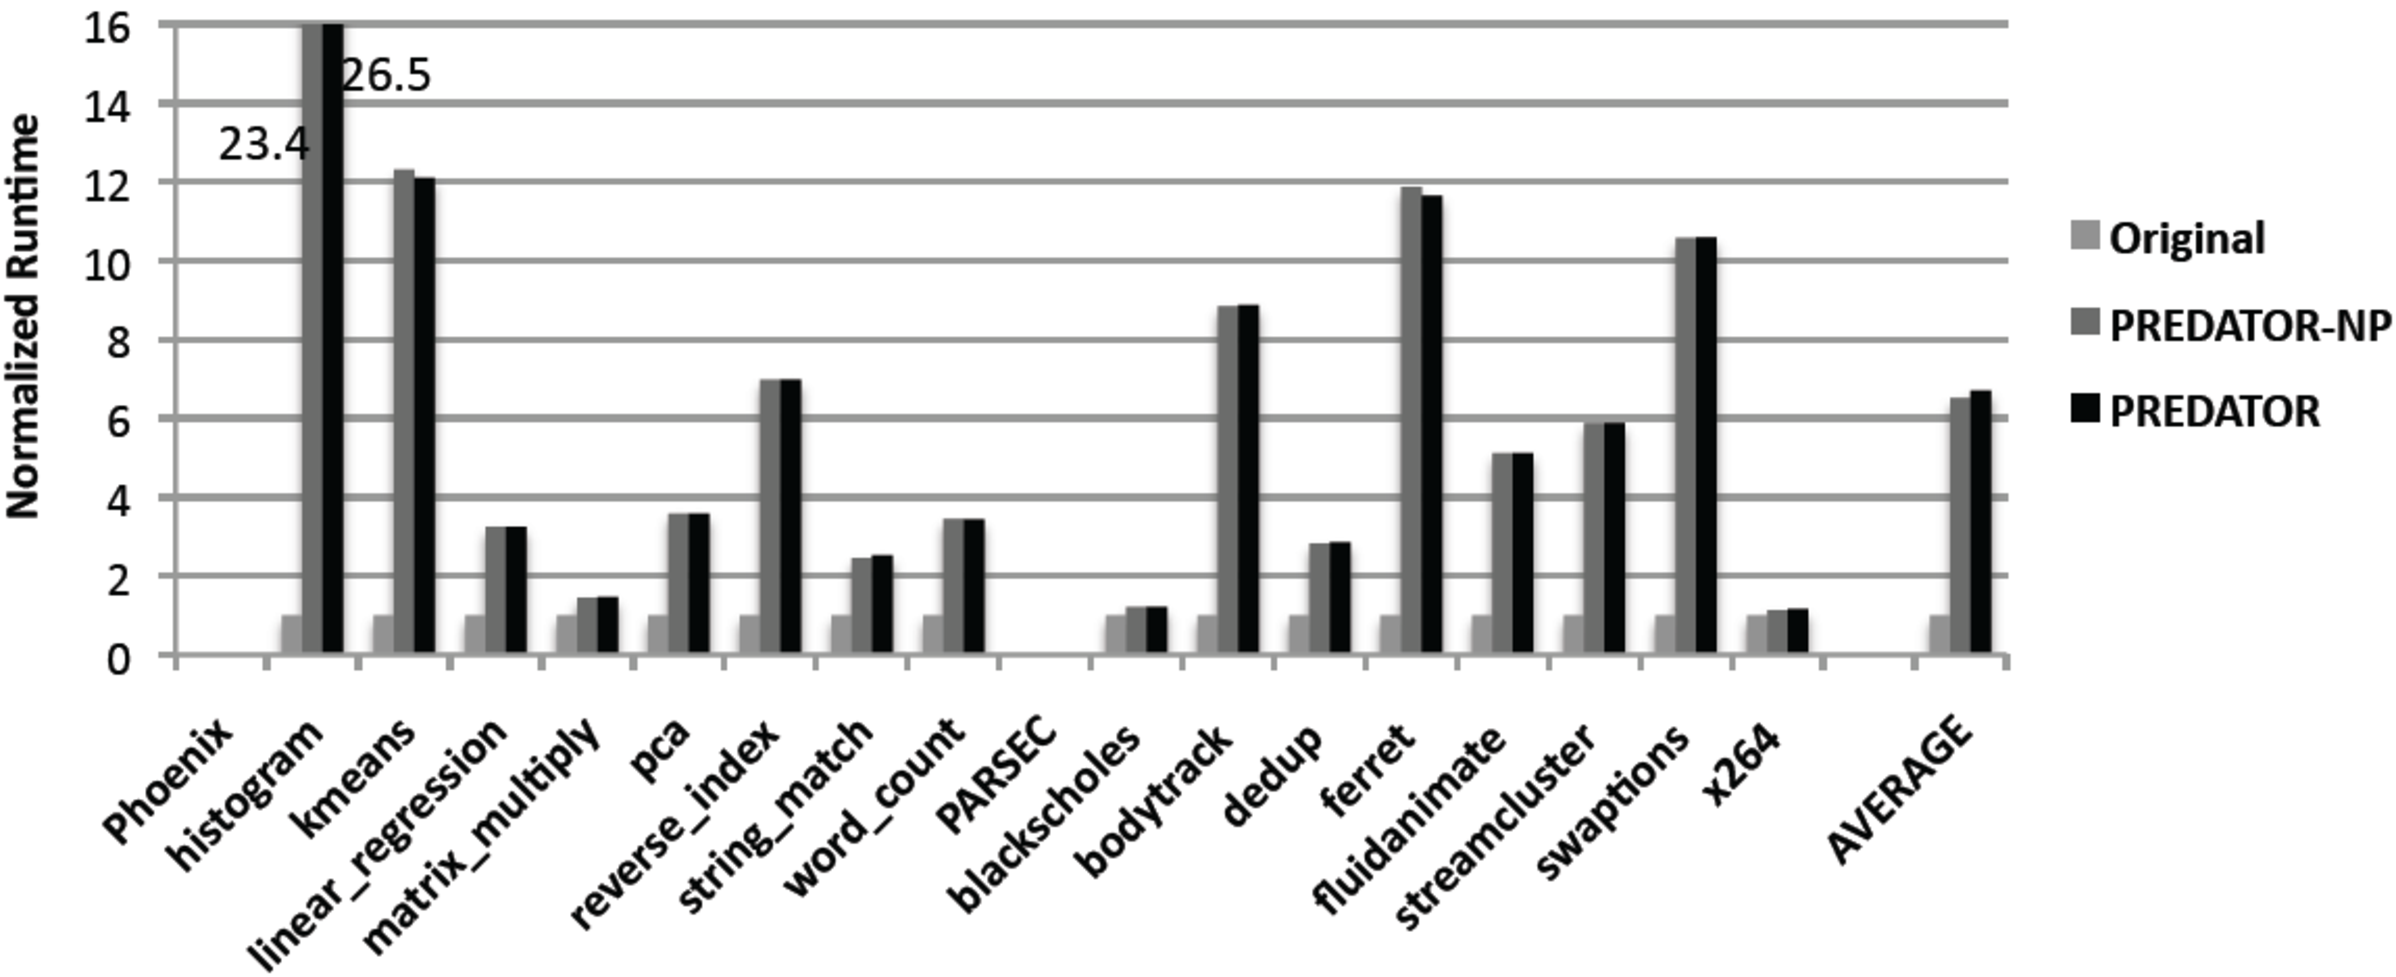
\includegraphics[width=6.5in]{fig/perf}
\end{center}
\caption{
Performance overhead of \Predator{} with and without prediction(PREDATOR-NP).
\label{fig:perf}}
\end{figure*}

To avoid the effect caused by extreme outliers, all performance data shown in this section
is based on the average of $10$ runs while excluding the maximum and minimum values.
Actual performance overhead with and without prediction 
can be seen in Figure~\ref{fig:perf}. 

From this figure, we can see for all $16$ benchmarks from Phoenix and PARSEC
benchmark suites that \Predator{} with prediction imposes around $6.7\times$
performance overhead. 
If we remove prediction from \Predator{}, we cannot observe significant performance difference.
This means that prediction of \Predator{} only introduces very minimum performance overhead. 

Among these programs, five of them have more than $8\times$ performance overhead, 
including \texttt{histogram, kmeans, bodytrack, ferret} and \texttt{swaptions}. 
Program \texttt{histogram} has the most performance overhead and 
runs more than $26$ slower than original executions. 
It has a severe false sharing problem inside, and tracking detailed access for those
problematic cache lines exacerbates the 
false sharing effect (see more discussion of this in Section~\ref{sec:sample}). 
For \texttt{bodytrack} and \texttt{ferret}, \Predator{} found a large amount of cache lines with 
writes larger than {\it Tracking-Threshold}. 
Tracking all accesses details for those cache lines 
imposes significant performance overhead. 
Currently, we have not identified the reasons 
why \texttt{kmeans} runs much slower in \Predator{}.   

In our evaluation, we do not observe significant performance overhead for
\texttt{matrix\_multiply, blackscholes} and 
\texttt{x264}.
In these, a large portion of the computation operates on stack variables, which are
not tracked by \Predator{}. 

\CC{ADD performance data on real applications}

\subsection{Memory Overhead}
\label{sec:memoverhead}
Since \Predator{} pre-allocates a huge block of memory
using \texttt{mmap} system call for its heap usage, 
virtual memory can not be used to evaluate actual memory overhead imposed by our tool. 
Hence, we only evaluate physical memory used for each application. 
According to the discussion of Justin et al.\ ~\cite{memusage}, proportional set size (PSS) 
in \texttt{/proc/self/smaps} is a suitable number since it reflects memory increase to the system
by running this application. 

To get PSS data, we start a script program to save 
corresponding \texttt{smaps} files periodically.
For each \texttt{smaps} file, we calculate the sum of PSSs for different
memory mappings and uses it as total physical memory usage for this application.
Among all collected \texttt{smaps} files, we choose the maximum value computed from
different files for comparison 
since it represents the maximum memory overhead to run this application.
%It is noted that we remove the physical memory usage of   
Results of maximum memory usage is shown in Figure~\ref{fig:memusage}. As we can see,
\Predator{} does not introduce substantial memory usage overhead 
for all evaluated benchmarks, except for \texttt{swaptions}. 
Removing \texttt{swaptions} from comparisons reduces 
the average memory overhead from 64\% to 22\%. 

The reason why \texttt{swaptions} introduces $7.8\times$ memory overhead is that 
its original memory usage is too small (only $3KB$).
Adding the code of detection, prediction and
reporting contributes to a large portion of memory overhead. 

\begin{figure*}
\begin{center} 
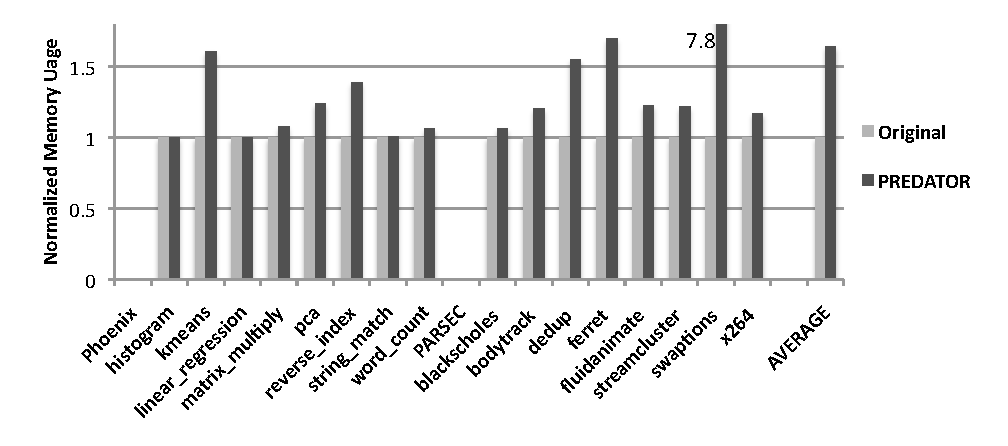
\includegraphics[width=6.5in]{fig/memusage}
\end{center}
%\includegraphics{fig/potential.pdf}
\caption{Memory usage overhead}
\label{fig:memusage}
\end{figure*}


\CC{NEW here.}
\subsection{Sensitivity on Sampling Rate}
\label{sec:sensitivity}
Different 
